\newpage
\section{Aufgabe 1: Mehrdimensionale Minimierung}
\label{sec:auf1}

\subsection{a)}
    Hier sollte die Intervallhalbierungsmethode implementiert werden.
    Es ist die Funktion
    \begin{equation}
        g(x, y) = x^2 + y^2 + x^2 y^2
    \end{equation}
    mit den zwei Sätzen von Anfangswerten
    \begin{equation}
        \vec{x} =
        \begin{pmatrix}
            1 \\ 0
        \end{pmatrix} \quad
        \vec{p} =
        \begin{pmatrix}
            -2 \\ 0
        \end{pmatrix} \;, \qquad \mathrm{und} \qquad
        \vec{x} =
        \begin{pmatrix}
            1 \\ 1
        \end{pmatrix} \quad
        \vec{p} =
        \begin{pmatrix}
            -2 \\ 0
        \end{pmatrix}
    \end{equation}
    gegeben.
    Zuerst wurde die Methode \verb|determineSupportingPoints()| implementiert, um die drei für die Intervallhalbierung nötigen Stützstellen grob zu bestimmen.

    Danach wird die Methode \verb|bisection()| für die beiden Anfangsbedingungen, bei einer Abbruchbedingung von $\epsilon = 10^{-7}$, durchgeführt und man erhält die lokalen Minima
    \begin{equation}
        \vec{x}_{\mathrm{min}} \approx 
        \begin{pmatrix}
            0 \\ 0
        \end{pmatrix} \; , \qquad
        \vec{x}_{\mathrm{min}} \approx 
        \begin{pmatrix}
            0 \\ 1
        \end{pmatrix} \; .
    \end{equation}
    


\subsection{b), c)}
    Beide implementierten Methoden konvergieren jeweils für alle drei Startwerte gegen $\begin{pmatrix}
        0 \\ 0
    \end{pmatrix}$.


\subsection{d)}
    Hier sollten die Minima der Funktion
    \begin{equation}
         f(x,y) = \left(1 + \frac{\exp(-10(xy-3)^2)}{x^2 + y^2}\right)^{-1}
    \end{equation}
    betrachtet werden.
    Das haben wir aber nicht mehr gemacht.

    \begin{figure}[H]
        \centering
        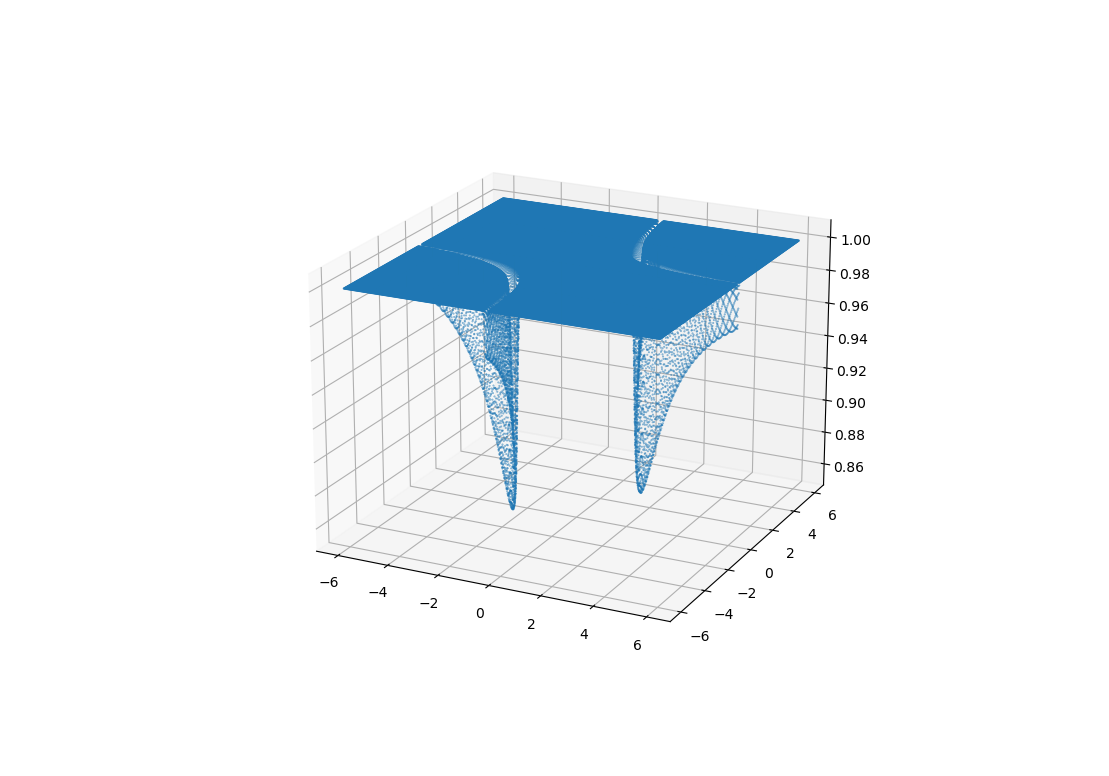
\includegraphics[width=1\textwidth]{pictures/function.png} \vspace*{-0.5cm}
        \caption{Hier ist die Funktion $f(x,y)$ aufgetragen.}
        \label{fig:function}
    \end{figure}
    \FloatBarrier
